\chapter{Grundlagen und Problembeschreibung}
\label{chapter2}
Bevor näher auf die verwendeten Algorithmen eingegangen wird,
werden grundlegende Aspekte erläutert.
Dabei werden neben einigen Interaktionsmodellen vor Wandbildschirmen
auch die eingesetzte Sensorik und die Struktur des Datensatzes beschrieben.
Zudem erfolgt abschließend eine ausführliche Problembeschreibung.


\section{Modelle der Interaktion mit Wandbildschirmen}
\label{2-ModelleInteraktion-Wandbildschirme}
Interaktive digitale Medien sind in der Öffentlichkeit immer präsenter.
Deshalb wird es für Wandbildschirme immer schwieriger die Aufmerksamkeit von Passanten zu erregen
und sie zur Interaktion zu animieren.
Diese Herausforderungen können nicht einfach durch verbesserte Hardware oder attraktivere Displays gelöst werden.
Stattdessen muss ein besseres Verständnis von Menschen und deren Technologienutzung geschaffen werden \citep{wouters_uncovering_2016}.
\emph{Ambient Displays} sind große, interaktive Bildschirme im (halb-) öffentlichen Raum, mit denen Nutzer interagieren können.
Es handelt sich meist um ästhetisch ansprechende Displays die Personen mit Informationen versorgen \citep{mankoff_heuristic_2003}.
Eine Kategorisierung der Interaktion von Personen mit solchen Wandbildschirmen kann das Verständnis des Verhaltens verbessern.
Dazu existieren verschiedenste \emph{Audience Behaviour-Interaktionsmodelle}, wovon im Folgenden zwei näher beschrieben werden.

Das \emph{Audience Funnel Modell} beschreibt, wie Menschen sich um ein großes öffentliches Display versammeln
und von Beobachtern zu Interagierenden mit dem System, und anschließend wieder zu Beobachtern werden.
Menschen neigen dazu verschiedene Phasen der Interaktivität zu durchlaufen,
bevor sie direkt mit dem System interagieren \citep{wouters_uncovering_2016, mai_audience_2018}.
Die einzelnen Phasen des \emph{Audience Funnel} werden in \autoref{fig:AudienceFunnelModel} gezeigt.
Eine der Aufgaben eines Wandbildschirms ist es also Aufmerksamkeit auf sich zu ziehen
und den Nutzer zu motivieren mit dem System zu interagieren \citep{mai_audience_2018}.
\citet{mai_audience_2018} verweisen darauf, dass \emph{Ambient Displays} in der Öffentlichkeit
nicht undbedingt der zentrale Punkt der Aufmerksamkeit sind, da vorbeigehende Personen eigene intrinsische Ziele verfolgen.
Die Herausforderung für Entwickler ist es die Systeme so zu gestalten,
dass sie Aufmerksamkeit erregen, sich aber gleichzeitig nicht gezwungen in den Mittelpunkt stellen.

\begin{figure}[ht]
    \begin{center}
    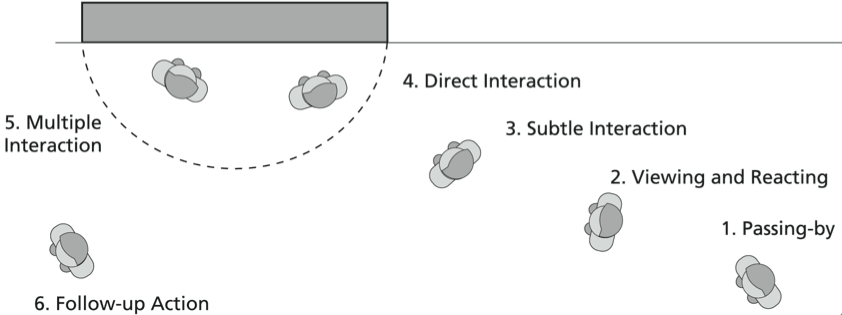
\includegraphics[width=0.8\textwidth]{audience-funnel-model.png}
    \end{center}
    \caption{Audience Funnel Framework. Abbildung aus \citet{mai_audience_2018}.}
    \label{fig:AudienceFunnelModel}
  \end{figure}

Ein zweites Modell wird durch den bereits erwähnten \emph{Honeypot-Effekt} beschrieben.
Er zeigt, dass Individuen undabhängig von Belohnungen, Bestrafungen oder sozialem Wettbewerb
von der reinen Präsenz oder den Aktivitäten anderer beeinflusst werden.
In der \ac{HCI} wird dies meist erkennbar, indem Passanten sich einem System nähern
und überlegen, ob sie mit ihm interagieren sollen,
nachdem sie anderen Menschen dabei zugesehen haben \citep{wouters_uncovering_2016}.

Eine Einordnung der Bewegungsdaten in die Kategorien solcher Modelle
und eine weiterführende Analyse der Bewegungen kann Aufschluss über das Verhalten von Menschen
vor interaktiven Bildschirmen geben.
Wie bereits erwähnt ist eine Kategorisierung des vorliegenden Kinect-Datensatzes
aufgrund der großen Datenmenge nicht manuell realisierbar.
Im Folgenden werden die Struktur des Datensatzes und die Grundlagen der verwendeten Sensorik beschrieben.
Aufbauend darauf werden Überlegungen angestellt,
wie eine Implementierung zur Automatisierung der Kategorisierung aussehen kann.


\section{Spezifikation der Kinect}
\label{2-SpezifikationKinect}
\citep{tolgyessy_evaluation_2021} verweisen darauf,
dass der Xbox 360 Kinect-Sensor eine \glqq Revolution\grqq\ im Bereich der erschwinglichen 3D-Erkennungssensorik war.
Ursprünglich war er für die Videospiel-Industrie gedacht.
Schon bald wurde er aber auch für wissenschaftliche Experimente genutzt.
In späteren Jahren folgten weitere Iterationen der Kinect \citep{tolgyessy_evaluation_2021}.
Im vorliegenden Datensatz des \emph{HoPE-Projekts} kam die Kinect v2 für Xbox One zum Einsatz.
Diese Sensorik stellt Farbbilder einer \ac{RGB} Kamera, Tiefenbilder einer Tiefenkamera
und Audiodateien verschiedener Mikrofone zur Verfügung \citep{windows-developer-center_microsoft_corporation_human_2014}.
Besonders die Tiefenkamera hilft zuverlässige Ergebnisse bei der Erkennung von Menschen vor \emph{Ambient Displays} zu erzielen.
\citet{li_time-flight_2014} fassen es wie folgt zusammen.
Die kompakte Größe, die Benutzungsfreundlichkeit,
die stark vereinfachte Hintergrund-Subtraktion im Vergleich zu anderer Sensorik, sowie die hohe Genauigkeit
und die hohe Bildrate machen Tiefenkameras zu einer attraktiven Lösung für ein breites Spektrum an Anwendungen.
Die Kinect v2 verwendet dabei den Ansatz der kontinuierlichen Wellenintensitätsmodulation,
der häufig bei \ac{ToF}-Tiefenkameras zum Einsatz kommt.
Dabei wird das Licht einer Lichtquelle von Objekten im Sichfeld der Kamera zurückgestreut
und die Phasenverzögerung zwischen dem emittierten und dem reflektierten Licht gemessen.
Diese Phasendifferenz wird für jedes Pixel im Bildfeld in einen Entfernungswert umgerechnet \citep{tolgyessy_evaluation_2021}.
Der Sensor kann Tiefenbilder mit einer Auflösung von 512 x 424 Pixeln
und gewöhnliche Farbbilder mit 1920 x 1080 Pixeln aufnehmen \citep{marin_multi-camera_2019}.
Bei der Kinect v2 können bis zu sechs Personen erfasst werden.
Dabei wird die Lage von 25 Skelettpunkten, sowie verschiedene Gesichtsattribute erfasst \citep{windows-developer-center_microsoft_corporation_human_2014}.
\autoref{fig:KinectBodyJoints} zeigt eine Übersicht dieser Punkte. 

\begin{figure}[ht]
  \begin{center}
  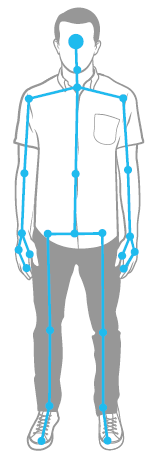
\includegraphics[width=0.1\textwidth]{kinect-body-joints.png}
  \end{center}
  \caption{Skelettpunkte der Kinect v2. Abbildung von \citet{windows-developer-center_microsoft_corporation_human_2014}.}
  \label{fig:KinectBodyJoints}
\end{figure}


\section{Struktur des vorliegenden Datensatzes}
\label{2-StrukturDatensatz}
Zur Evaluation des implementierten System dienen verschiedene Teilmengen des Kinect-Datensatzes des \emph{HoPE-Projekts}.
Hierfür wurden im Jahr 2017 für 18 Wochen \emph{Ambient Displays} mit Kinect v2 Systemen ausgestattet.
Zu erwähnen ist zudem, dass das entwickelte Tool zur Auswertung auch mit anderen Datensätzen funktionieren soll.

Eine Auswertung des Datensatzes ergab, dass dieser 97.626 Records beinhaltet \citep{temiz_konzeption_2022}.
Dabei enthält jeder mehrere sogenannte Frames.
Dabei handelt es sich um Momentaufnahmen der Kinect-Sensorik.
Falls sich mehrere Menschen gleichzeitig im Sensorbereich befinden,
erhält jede Person eine eindeutige Identifikationsnummer
und der Record wird in mehrere Frames unterteilt.
Dabei entspricht ein Frame der Momentaufnahme einer Person.
Zu jedem Record liegen verschiedene Dateien vor,
die jeweils den Zeitstempel in Kombination mit einem geeigneten Postfix als Dateinamen tragen.
\autoref{tbl:AttributesDataset} zeigt die Attribute der Datei \emph{timestamp.txt}.
\begin{table}[ht]
  \begin{center}
    \begin{tabular}{ |c|c| } 
      \hline
      Attributname & Beschreibung \\
      \hline \hline
      Zeitstempel & Zeitpunkt der Aufnahme \\
      \hline
      KinectId & Skelett-Identifikationsnummer des Framework  \\
      \hline
      RecordId & Identifikationsnummer des Records \\
      \hline
      BodyIndex & Identifikationsnummer der Person \\
      \hline
      BodyCount & Anzahl der erfassten Personen \\
      \hline
      Happy & Person ist glücklich \\
      \hline
      Engaged & Person zeigt Interesse \\
      \hline
      WearingGlasses & Person trägt eine Brille \\
      \hline
      LeftEyeClosed & Person hat das linke Auge geschlossen \\
      \hline
      RightEyeClosed & Person hat das rechte Auge geschlossen \\
      \hline
      MouthOpen & Person hat den Mund geöffnet \\
      \hline
      MouthMoved & Person bewegt den Mund\\
      \hline
      LookingAway & Person schaut nicht zur Kinect \\
      \hline
      Body.HandLeftState & Zustand der linken Hand \\
      \hline
      Body.HandRightState & Zusand der rechten Hand \\
      \hline
      x & x-Koordinate des Skelettpunkts SpineShoulder \\
      \hline
      y & y-Koordinate des Skelettpunkts SpineShoulder \\
      \hline
      z & z-Koordinate des Skelettpunkts SpineShoulder \\
      \hline
      Distance & Distanz zwischen Kinect und Skelettpunkt SpineShoulder \\
      \hline
    \end{tabular}
    \caption{Attribute des Datensatzes.}
    \label{tbl:AttributesDataset}
  \end{center}
\end{table}
Diese Attribute werden in der Textdatei durch drei Rauten ('\#\#\#') voneinander abgegrenzt.
Ein konkreter Frame aus dem Datensatz kann \autoref{fig:FrameExample} entnommen werden.

\begin{center}
\begin{figure}[ht]
    2017-04-10 07:41:53.943 +02:00 \#\#\# 72057594038063128 \#\#\# 1341053376 \#\#\# 1 \#\#\#
    \newline 1 \#\#\# No \#\#\# Maybe \#\#\# Unknown \#\#\# No \#\#\# No \#\#\# No \#\#\# Yes \#\#\#
    \newline Maybe \#\#\# Unknown \#\#\# Closed \#\#\# 0,1074784 \#\#\# 0,2451882 \#\#\# 4,18441 \#\#\#
    \newline 4,19296454679429
    \caption{Frame aus dem Datensatz.}
    \label{fig:FrameExample}
  \end{figure}
\end{center}

Da die Anordnung und das Vorhandensein dieser Attribute je nach Version des Datensatzes abweichen kann,
sollen diese in der Implementierung manuell konfigurierbar sein.
Die Datei \emph{timestamp$\_$bodies.txt} enthält für jeden Frame die Position aller 25 Skelettpunkte.
\emph{timestamp$\_$summary.txt} zeigt eine kurze Zusammenfassung des Records, welche gut menschenlesbar ist.
\emph{timestamp.xef} kann genutzt werden, um die Aufnahme in der Anwendung Kinect Studio zu visualisieren.
Letztlich sind die Einträge sogenannte \emph{\ac{TSD}}.
Bei diesem Datentyp handelt es sich um geordnete Sequenzen von Datenpunkten,
die über eine gewisse Zeit hinweg aufgenommen wurden.
Oft in regelmäßigen Abständen \citep{ali_clustering_2019}.
Insgesamt befinden sich im Datensatz 34.687.630 Frames \citep{temiz_konzeption_2022}.
Diese Anzahl bestätigt erneut die Notwendigkeit eines Software-Tools zur Auswertung.
Um aussagekräftige Ergebnisse zu erhalten lohnt es sich gegebenenfalls mit Teilmengen des Datensatzes zu arbeiten.
So liefern beispielsweise Records mit weniger als zwei Sekunden zu wenig Information
für Erkenntnisse über das Interaktionsverhalten.
So werden auch in \autoref{chapter6} bereits gefilterte Teilmengen des gesamten Datensatzes
zur Evaluation verwendet.
Je nach Fragestellung kann es ebenfalls lohnenswert sein Records mit einer, zwei oder mehreren Personen
gesondert zu betrachten.

\section{Problembeschreibung}
\label{2-Problembeschreibung}
Es gibt verschiedene Möglichkeiten sich der Kategorisierung von Bewegungsdaten zu nähern.
So kann beispielsweise \emph{Maschine Learning} eingesetzt werden.
Dieser Ansatz wird derzeit ebenfalls im Rahmen des HoPE-Projekts erforscht \citep{plischke_master_2022}.
In dieser Bachelorarbeit werden hingegen \emph{deterministische Algorithmen} genutzt.
Durch sie kann die Implementierung eines Kategorisierungssystems verhältnismäßig einfach gehalten werden.
\citet{aghabozorgi_time-series_2015} verweisen zudem darauf, dass die Verwendung von Methoden
wie Maschine Learning (\emph{supervised}), im Falle von großen Datensätzen zu Problemen führen kann.
Deterministische Cluster-Algorithmen sollten bei großen Datenmengen weniger Probleme bereiten (\emph{unsupervised}).

Beim vorliegenden Kinect-Datensatz handelt es sich ebenfalls um eine große Datenmenge.
Die einzelnen Records müssen daher automatisiert bearbeitet werden.
Ziel der Verarbeitung ist es möglichst sinnvolle \emph{Cluster} zu erhalten.
Um die Gemeinsamkeiten zweier Aufnahmen zu berechnen,
wird eine geeignete Vergleichsfunktion benötigt.
Die Wahl dieser Funktion ist wichtig für den Erfolg des \emph{Clusterings} \citep{warren_liao_clustering_2005}.
Zu beachten ist zudem, dass die Bewegungsaufnahmen durch \emph{\ac{TSD}} beschrieben werden.
Werden hier herkömmliche Distanzmetriken, wie die Euklidische-Distanz verwendet
kann dies zu Problemen führen und die Aussagekraft des Vergleichs verringern.
Es kann vorkommen, dass verschiedene Personen die gleiche Bewegung unterschiedlich schnell,
oder zeitlich versetzt ausführen.
Gegebenenfalls weisen die Datenreihen bei der gleichen Bewegung daher sogar eine unterschiedliche Anzahl an Frames auf.
\autoref{fig:MetricComparison} zeigt ein exemplarisches Szenario.
Die Kurven weisen ähnliche Segmente auf.
Sie sind allerdings unterschiedlich lang und die Ähnlichkeiten treten zu unterschiedlichen Zeitpunkten auf.
Mit der bekannten euklidischen Distanz ist das Ergebnis hier nicht aussagekräftig
und der letzte Punkt der Reihe kann gar nicht zugordnet werden.
Um dieses Problem zu lösen ist eine elastische Metrik nötig,
die besser mit zeitlichen Verschiebungen umgehen kann \citep{aghabozorgi_time-series_2015}.

\begin{figure}[ht]
    \begin{center}
    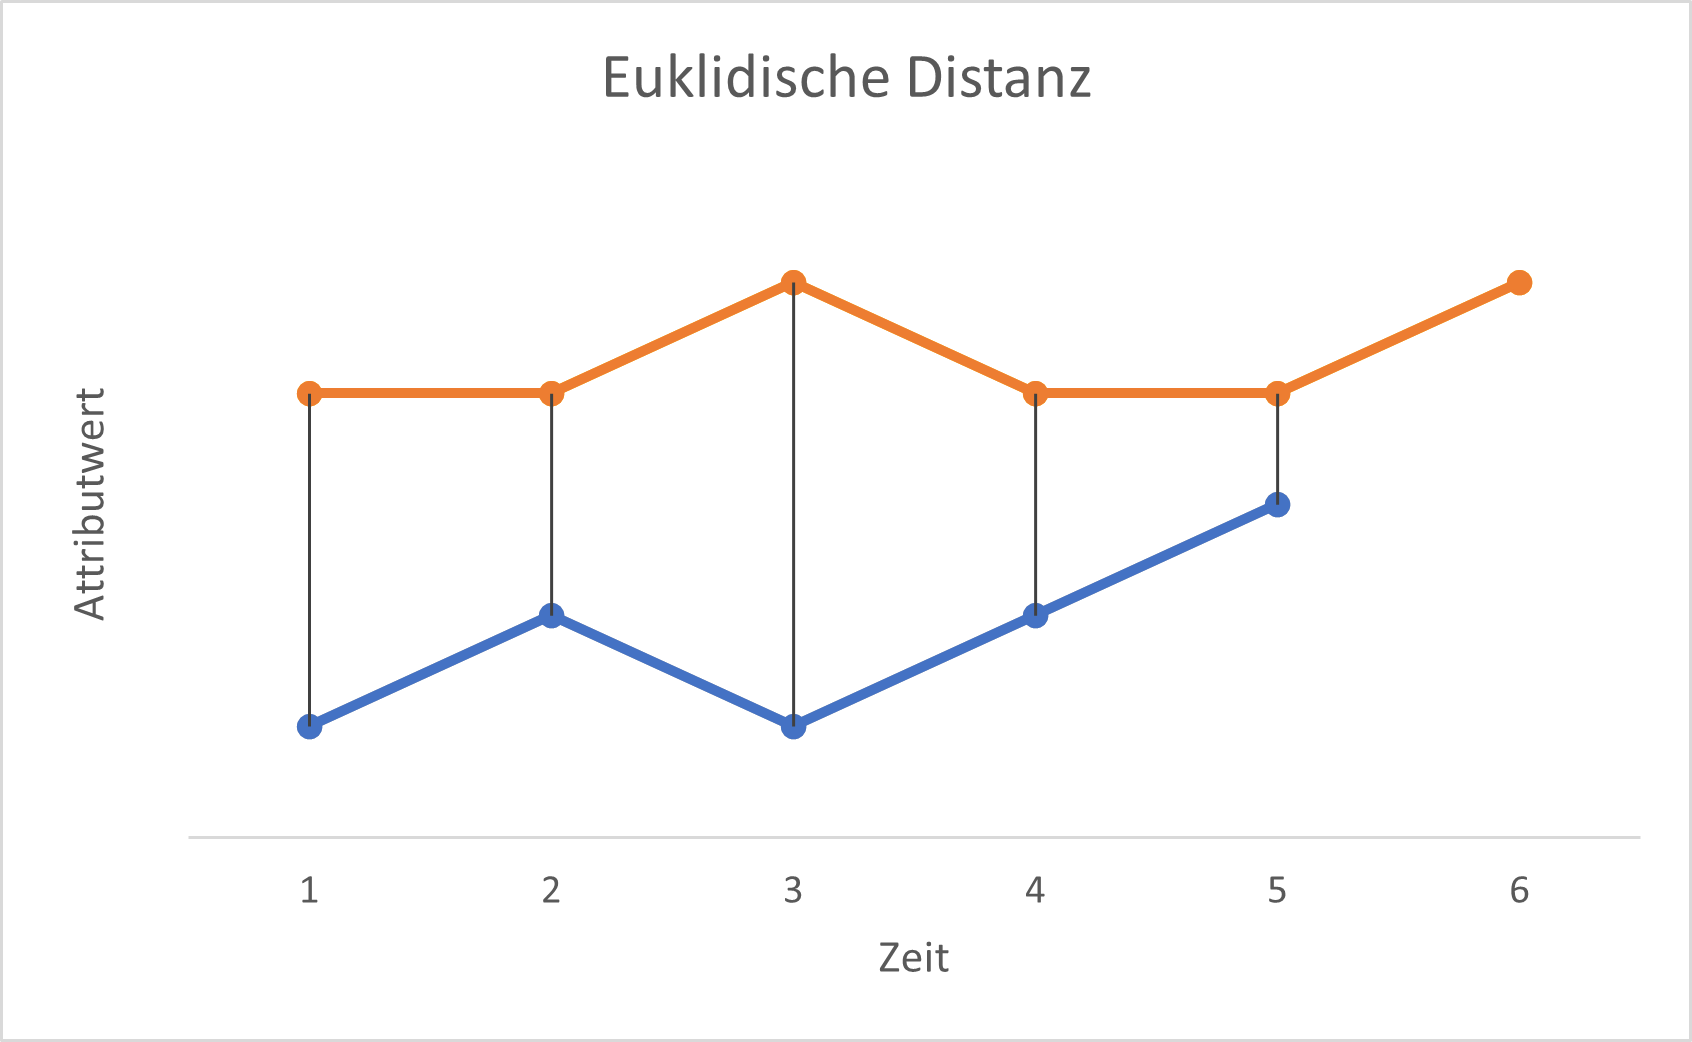
\includegraphics[width=0.45\textwidth]{EuclidianMetric.png}
    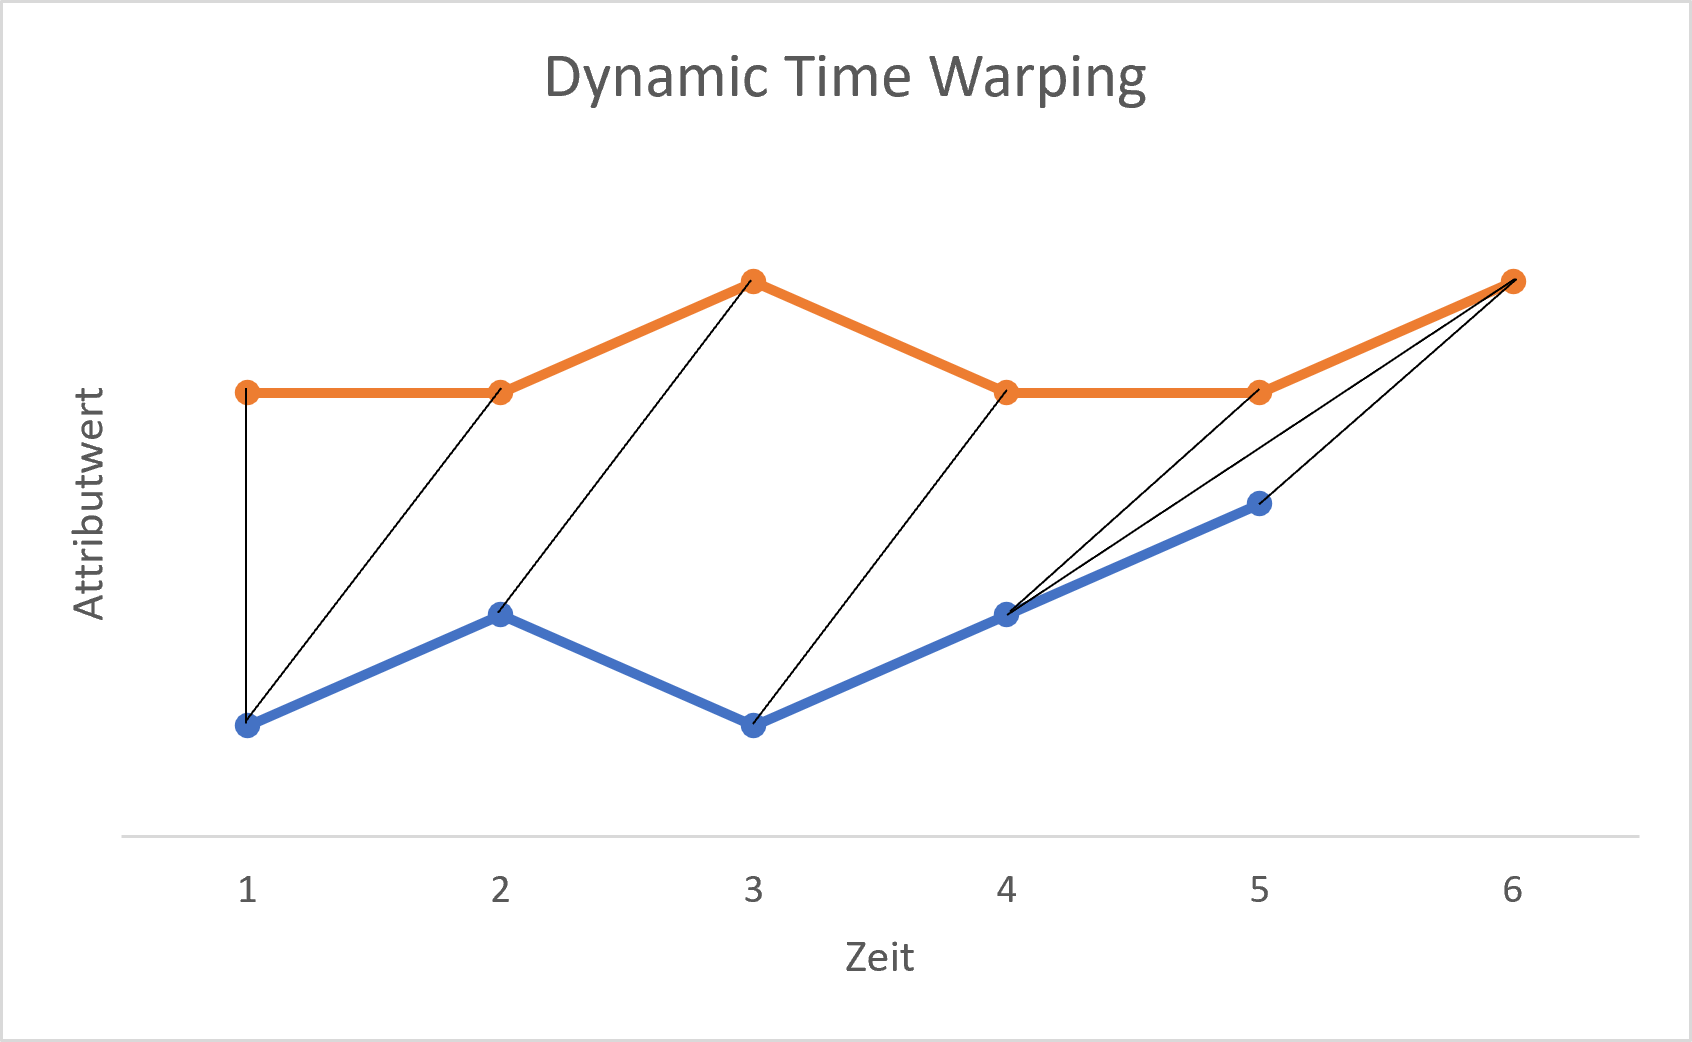
\includegraphics[width=0.45\textwidth]{DTWMetric.png}
    \end{center}
    \caption{Zuordnung der Messpunkte zweier Datenreihen.}
    \label{fig:MetricComparison}
\end{figure}

Das Clustering soll mithilfe von \emph{hierarchischem Clustering} durchgeführt werden,
welches in \autoref{3-Clustering} beschrieben wird.
Das Verfahren ist für die vorliegenden Daten gut geeignet,
da es erlaubt \ac{TSD} unterschiedlicher Länge zu clustern.
Zudem muss die Anzahl der zu bildenden Cluster nicht im Voraus definiert werden,
wie dies etwa bei \emph{K-Means} der Fall ist \citep{aghabozorgi_time-series_2015}.
Es ist in diesem Kontext nicht zielführend die Clusteranzahl zuvor zu definieren,
da die Arbeit darauf abzielt, mehr Erkenntnis über mögliche sinnvolle Cluster zu gewinnen.
Statt die Anzahl vorzugeben, wird ein Threshold definiert der angibt,
ab wann zwei Cluster nicht mehr zusammengeführt werden soll,
weil die Differenz zwischen ihnen zu groß ist.
Als geeignete Distanz-Metrik wird dabei \emph{\ac{DTW}} verwendet (\autoref{3-DTW}).
Hier ist eine Mehrfachzuordnung von Punkten möglich.
Diese können so verbunden werden, dass die Kosten minimal sind.
Dies erlaubt eine Zuordnung ähnlicher Muster in den Daten auch wenn sie zeitlich verschoben sind
und ist daher gut für unsere Problemstellung geeignet.